% !TEX root = DataDrivenBayes.tex


\section*{Case study 2: Using descriptive models to complement optimal ones} 

The previous case study presented a situation in which an optimal Bayesian model a descriptive model ended up in conflict: The optimal model was inconsistent with the empirical data, and it was the descriptive model that shed light on how people approached the task. This is perhaps to be expected whenever human cognition genuinely departs from a normative standard. However, the interaction between these two perspectives need not always be antagonistic, and our second case study illustrates a situation where a descriptive Bayesian approach is complementary to the optimal Bayesian approach, and ultimately reinforces the conclusions that an optimal model produces.




%To motivate this study, we begin by noting that our previous case study compared two different Bayesian models and yielded psychological insights that seemed intuitively reasonable. However, it is entirely possible that we could have arrived at equally reasonable inferences had we used alternative cognitive models---perhaps even non-Bayesian ones. Moreover, our model evaluation was at best qualitative: We noted that the original model failed to capture key qualitative patterns in the data that the more descriptive model could easily fit. There are many situations in which this is an appropriate way to compare models, and indeed there are statistical procedures that aim to formalize qualitative model comparison \cite<e.g.,>{pitt_global_2006}. However, it is often important to make quantitative model comparisons as well as qualitative ones. Insofar as the descriptive approach argues that Bayesians should build more flexible and hence more statistically complex models it is important that we also advocate that Bayesian cognitive modellers use model evaluation methods that take this complexity into account  \cite<e.g.,>{myung_importance_2000}. 
%
%There are many such data analysis tools, but for our purposes we will discuss the use of cross-validation \cite<e.g.>{browne_cross-validation_2000} when applied to an optimal Bayesian model, a descriptive Bayesian model, and a non-Bayesian heuristic model. The goal is to demonstrate that quantitative comparison between different kinds of models is not only possible within the descriptive framework, but also that such comparison can be more revealing than any single model taken alone.

\subsection*{Optimal predictions in everyday cognition}

Our second case study focuses on work by \citeA[henceforth GT2]{Griffiths2006} focusing on the question of whether human predictions in very simple inductive problems are genuinely optimal. To investigate this question, they gave people problems similar to the following one:
\begin{quote}
{\it If you were assessing the prospects of a 60-year-old man, how much longer would you expect him to live?}
\end{quote}
This problem can be characterized as form of Bayesian inference in which it is possible to rely on external sources to specify a veridical prior. For instance, actuarial statistics can be consulted to estimate $P(t)$, the prior probability that a randomly selected (American) man will die at age $t$; all of the problems considered by GT2 (movie grosses, poem lengths etc) had this property. Moreover, the evidence $x$ specified in the problem (i.e., the fact that this man has reached age 60) is not especially complicated, and suggests a very simple likelihood function. If the learner assumes that they have encountered this person at a randomly chosen moment in their life, then the probability that a person who lives to age $t$ will be encountered at age $x$ is simply
\begin{equation}
P(x \mid t) = \left\{ \begin{array}{rl} 1/t & \mbox{ if } x\leq t \\ 
0 & \mbox{ otherwise} \end{array} \right.
\end{equation}
To determine the eventual lifespan for someone observed to be alive at age $x$, we apply Bayes' rule. The posterior probability that the person lives to age $t$ is given by
$
P( t \mid x ) \propto P(x \mid t) P(t)
$.
As noted by GT2, the optimal answer to the prediction problem is to report the median of the posterior distribution over $t$, but in light of more recent work arguing that people can make near-optimal decisions by taking a small number of samples from the posterior \cite{vul_one_2014} we use a probabilistic version of the GT2 model that generates responses by sampling $t$ from the posterior $P(t \mid x)$.

The critical theoretical point that GT2 made was that this model can be used as a genuine normative standard for human cognition, since it uses veridical priors and well-motivated likelihoods. It therefore involves no free parameters that need to be estimated from the data. To the extent that human performance matches the predictions of this model, a strong case can be made that it is genuinely optimal. 


\subsection*{A descriptive but non-optimal Bayesian model}

The model proposed by GT2 represents one of the best developed examples of a Bayesian model that genuinely meets the requirements of an optimal model. It is therefore worth contrasting the GT2 model with a descriptive Bayesian model that explicitly avoids making any claim that people have veridical prior knowledge and instead aims merely to describe the empirical data. As with our previous example, we start from a position of researcher uncertainty: Instead of assuming that people's priors match the veridical ones, we treat people's subjective priors as unknown variables and seek to infer them from the empirical data.  

There are three attractive features to this approach. First, it seems plausible to think that at least some participants will have little knowledge of the statistics of the environment, and when asked to solve a prediction problem they will substitute some other distribution $P(t)$ in place of the true one. Second, by specifying the model in a less restrictive way, we can use it as a tool to learn something the prior distributions people use to solve simple inference problems.  Third, it expands the range of prediction problems that we can present to participants: There are many problems for which people seem to be able to give sensible sounding answers where no veridical prior distribution exists (e.g., how long will people live in the year 2100?). By treating the participant prior as a quantity to be learned rather than pre-specified by the researcher, we can use the Bayesian model as a tool to explore people's beliefs about these scenarios. 

The model we use is identical to the probabilistic version of the optimal predictions model described above in all respects except for the prior.\footnote{We could also naturally perform inference over people's likelihoods as we did in case study 1, and a full descriptive Bayesian model would do so. We choose not to here for expository purposes, since the purpose of the case study is to focus on comparing models and demonstrating the utility of making inferences about the priors specifically.} In the original GT2 model, the prior was constrained to be veridical. In the descriptive version we adopt an exploratory, data driven approach and consider a broad family of possible prior distributions that people might have relied upon when making judgments.  There are a number of ways that we could go about this. For instance, we could adopt a nonparametric Bayesian approach \cite<e.g.,>{griffiths_categorization_2008} and specify a very broad family of priors. 
However, as GT2 noted, for most of the problems of interest the veridical prior could be captured by a normal, Erlang or Pareto distribution. With that in mind our model assumes that for any given prediction problem, each participants relies on one of these three distributions.
\footnote{By limiting the space of priors in our model to normal, Erlang, and Pareto we are bringing in our priors (as researchers) about the family of distributions that describe people's priors based on what we previously learned in GT2. This allows us to do a more constrained learning about people's priors and serves to simplify our analysis somewhat. As mentioned in the main text, we could have used a much more flexible nonparametric prior but this would have reflected a researcher prior suggesting that people's knowledge about events was equally likely to take any number of more complex forms. A case could be made for this more flexible approach --- particularly if we had included other phenomena such as GT2's cake baking times which are multimodal. For our purposes, however, we chose a more constrained model because it still allowed us to answer the psychological questions of interest while remaining relatively simple to understand --- the nonparametric approach would introduce a level of technical complexity to our model that would distract from the important points of the case study.}
Unlike GT2, we do not pre-specify which distributions are used to solve which problems, nor do we make strong assumptions about the parameter values that describe the priors.
The technical details are discussed in Appendix B. What is important is that (a) our model does not assume that people make optimal predictions because it does not assume that people rely on veridical priors and (b) our model is more statistically complex than the one developed by GT2 because there are many possible priors that are consistent with this model. Because we did not place very strong constraints on what priors participants might have used, any analyses conducted using it are more exploratory and data-driven. %One might wonder, therefore, whether this new Bayesian model will serve any useful purpose when applied to empirical data. It clearly does not correspond to any claim about optimality. Moreover, 
  

\subsection*{A non-Bayesian alternative: the \mink heuristic}

So far we have considered two Bayesian models: the optimal predictions model of GT2 and our descriptive alternative. However there are of course other possibilities. One such possibility is the \mink heuristic, which was proposed by \citeA{Mozer2008} as an alternative non-Bayesian account of the prediction task. The model assumes that people not only have limited knowledge (analogous to the subjective priors of our descriptive model). It also assumes that people apply non-Bayesian decision rules to make their judgments. Specifically, it proposes that for each phenomenon, people have a small number ($k$) of exemplars in memory. The idea is that these exemplars represent a set of recalled events that are sampled from the prior, but this impoverished representation is the only knowledge that people have to guide their judgments. 

The \mink model also specifies a deterministic response rule for predicting the extent or duration of an event: respond with the smallest of the $k$ exemplars that is larger than the probe value $x$. If the probe is larger than all of the exemplars, then respond with a value that is larger than $t$ by a constant proportion $g$. If $e$ denotes the values of the set of stored examples, then the \mink model predicts that
\begin{equation}
t =
\left\{
\begin{array}{l l}
	x(1+g) & \quad \text{if } x>\max{e}\\
	\min{\left\{{y \in e \mid y>x}\right\}} & \quad \text{otherwise}\\
\end{array} \right.
\end{equation}
In our applications, we follow \citeA{Mozer2008} and adopt the version of the model in which the exemplar set $e$ consists of only $k=2$ items sampled from the true prior distribution. However, in order to make the model comparable to the two Bayesian models described above (both of which assume people respond probabilistically) we developed a variant of the model that we refer to as the ``Noisy \mink'' model that introduces response error and also assumes that the exemplars $e$ and multiplier $g$ are unknown quantities to be inferred from data (rather than a value fixed at 3). Again, the technical details are discussed in Appendix B.

\subsection*{Replicating and extending the GT2 study}

To compare the three models we ran a replication and extension of the GT2 study, in which we asked participants the same questions used in the GT2 study as well as a counterfactual question for which no true environmental statistics exist. Participants were 25 undergraduates from the University of California, Irvine who were compensated with partial course credit. Questions were presented to participants through a web-based survey. There were eight different question types and five variations of each question; each person saw all 40 questions in a random order. Each variation corresponded to one of five possible values of $x$. Only one question was presented on-screen at a time and participants entered their answer in a text-entry box before moving to the next question.

The survey instructions and seven of the questions were identical to those used by GT2. For the unabbreviated questions and survey instructions, refer to \citeA{Griffiths2006}. Below are abbreviated examples of each of the questions with all five of the possible values included:
\begin{description}[noitemsep]\setlength{\itemindent}{-.2cm}
\item[Lifespans:] {\it Predict the age a man will live to if he is currently (18, 39, 61, 83, 96) years old.}
\item[Movie grosses:] {\it Predict what the total box-office intake for a movie that has taken in (\$1, \$6, \$10, \$40, \$100) million so far.}
\item[Movie runtimes:] {\it Predict the length of a movie that has already been playing for (30, 60, 80, 95, 110) minutes.}
\item[Poem lengths:] {\it Predict the total length of a poem from which you were just quoted line (2, 5, 12, 32, 67).}
\item[Pharaohs' reigns:] {\it Predict the total time a pharaoh will be in power if he had already reigned for (1, 3, 7,11, 23) years in 4000 BC.}
\item[Representatives' terms:] {\it Predict the total years that a (1, 3, 7, 15, 31) year member of the U.S. House will serve.}
\item[Waiting times:] {\it Predict how long you will be on hold if you have already been holding on the phone for (1, 3, 7, 11, 23) minutes.}
\end{description}
The counterfactual question that was not part of GT2's study was:
\begin{description}\setlength{\itemindent}{-.2cm}
\item[Future lifespans:] {\it Suppose it is the year 2075 and medical science has advanced significantly. You meet a man that is (18, 39, 61, 83, 96) years old. To what age will this man live?}
\end{description}
Responses from each participant were considered for exclusion based on each question type: If any of a person's responses for one of the eight question types were below the value of $x$ that was presented in the question, then all five of that participant's responses for that question type were excluded for analysis. However, their responses for other question types were still included. %---as long as they passed the inclusion requirement above. AP: what does this refer to?
The number of participants that were included in the analysis for each question type were: 24 for life spans; 23 for box office intake; 23 for movie duration; 25 for poem lengths; 24 for pharaohs' reigns; 20 for U.S. representatives' terms; and 25 for future lifespans.


\subsection{Results}

%The results of our replication are shown in Figure~\ref{fig:emp_vs_mink_agg_predictive}, and are generally in agreement with the original experiment. 
%\bigskip

\subsubsection{Descriptive adequacy}

When evaluating the models, a common approach is to plot model predictions against human data and assess whether the model captures the qualitative pattern of human responses. A model that cannot reproduce the basic patterns observed in empirical data can be ruled out as a plausible theory of human behavior. However, as shown in Figure~\ref{fig:emp_vs_mink_agg_predictive}, all three models meet this basic criterion of descriptive adequacy. To determine which model fits best, we follow \citeA{Mozer2008} and use the normalized root mean squared error (NRMSE) between the median predictions of each model and the median human responses. The model fits are reported in Table~\ref{tbl:nrmse_comparison} and agree with the visual inspection: The Noisy \mink model fits the data better than either of the Bayesian models, although all fit reasonably well. 


\begin{figure}
	\makebox[\linewidth][c]{%	
	\begin{subfigure}{.33\textwidth}
		\caption{Movie grosses}
		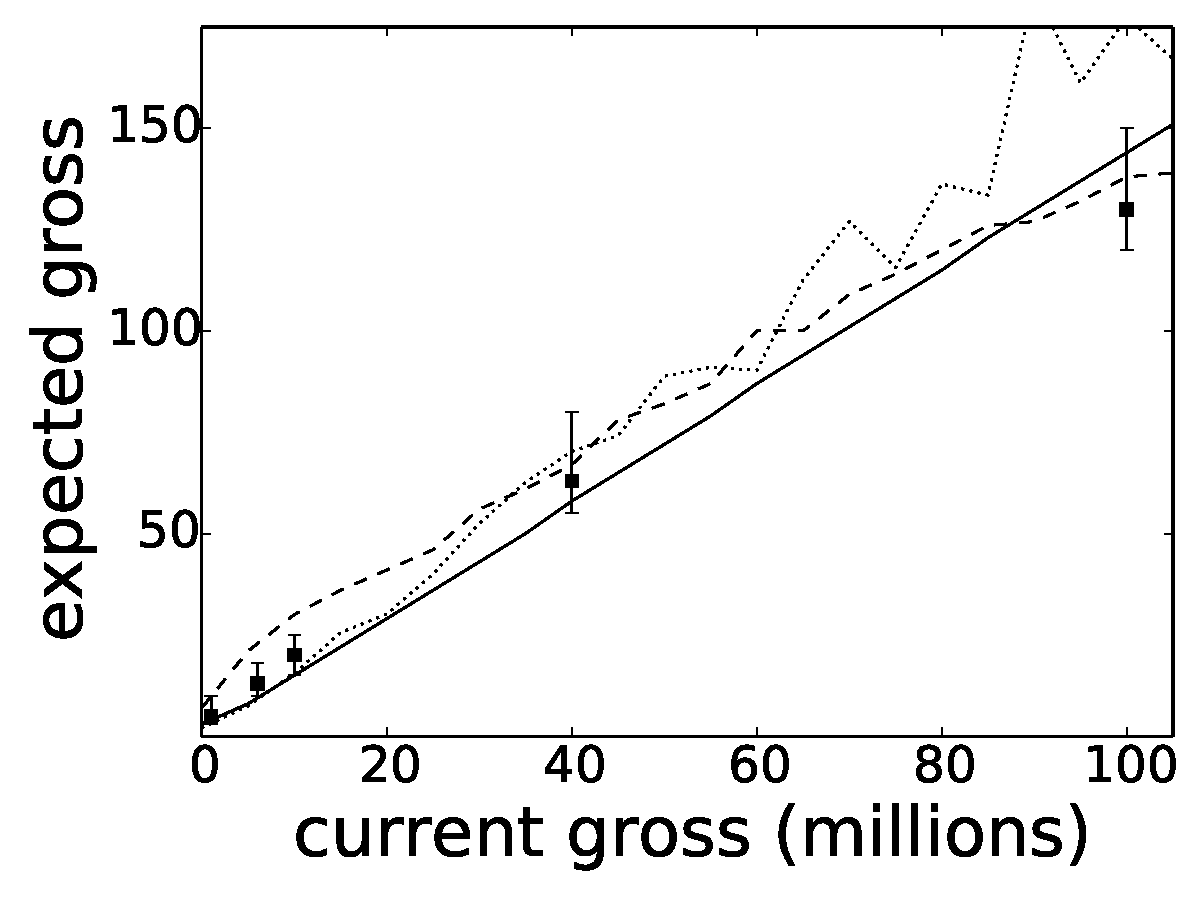
\includegraphics[width=1.0\textwidth]{predictions_figures/movie_grosses_pred.pdf}
	\end{subfigure}
	\begin{subfigure}{.33\textwidth}
		\caption{Poem lengths}
		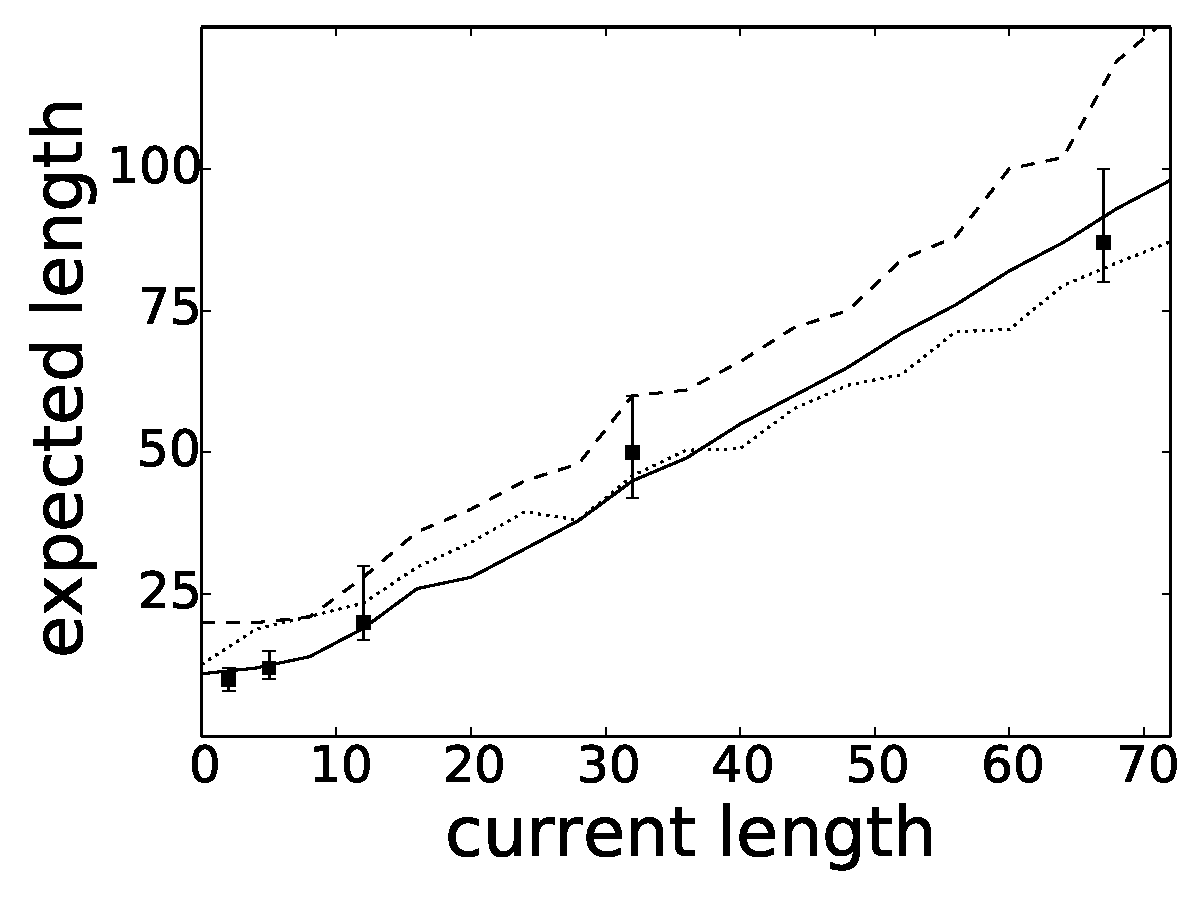
\includegraphics[width=1.0\textwidth]{predictions_figures/poem_lengths_pred.pdf}
	\end{subfigure}
	\begin{subfigure}{.33\textwidth}
		\caption{Lifespans}
		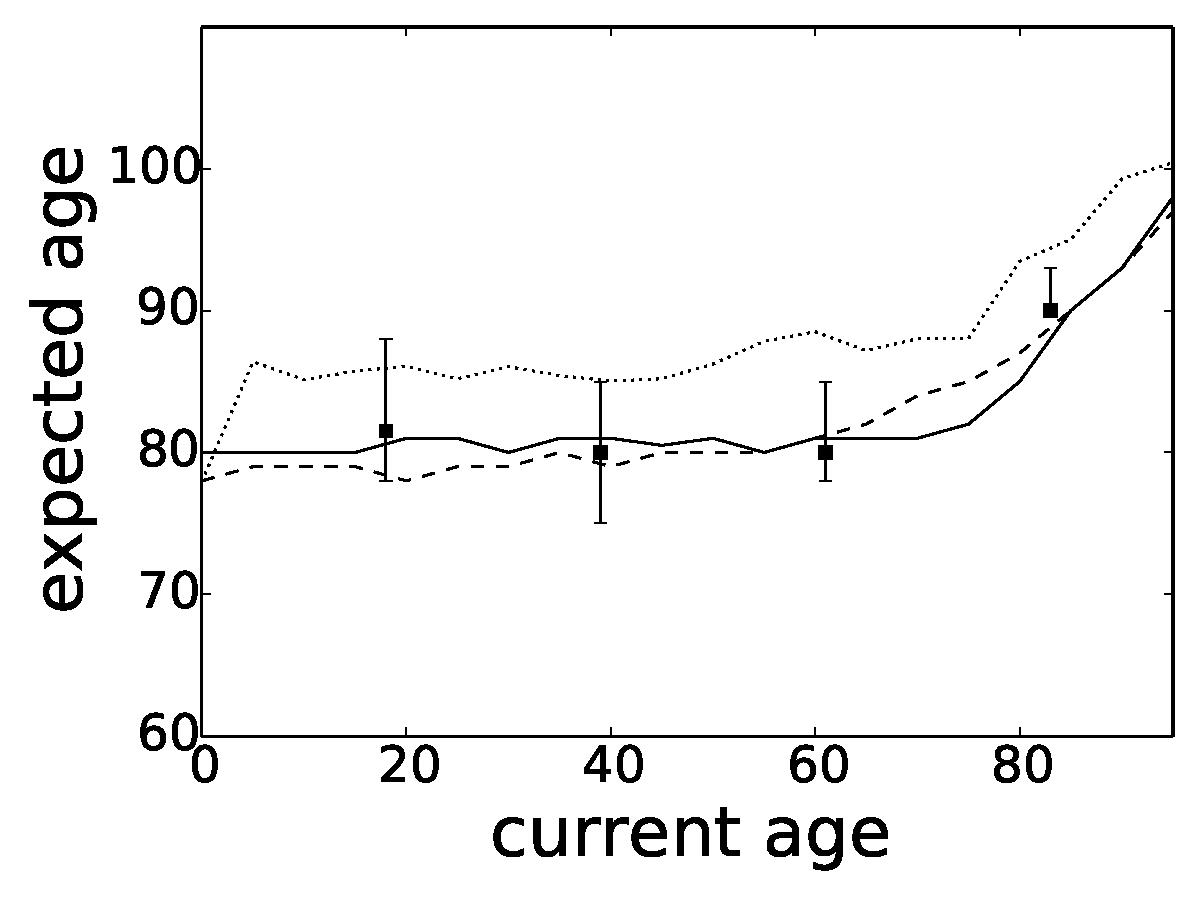
\includegraphics[width=1.0\textwidth]{predictions_figures/life_spans_pred.pdf}
	\end{subfigure}
	}\\
	\makebox[\linewidth][c]{%	
	\begin{subfigure}{.33\textwidth}
		\caption{Pharaohs}
		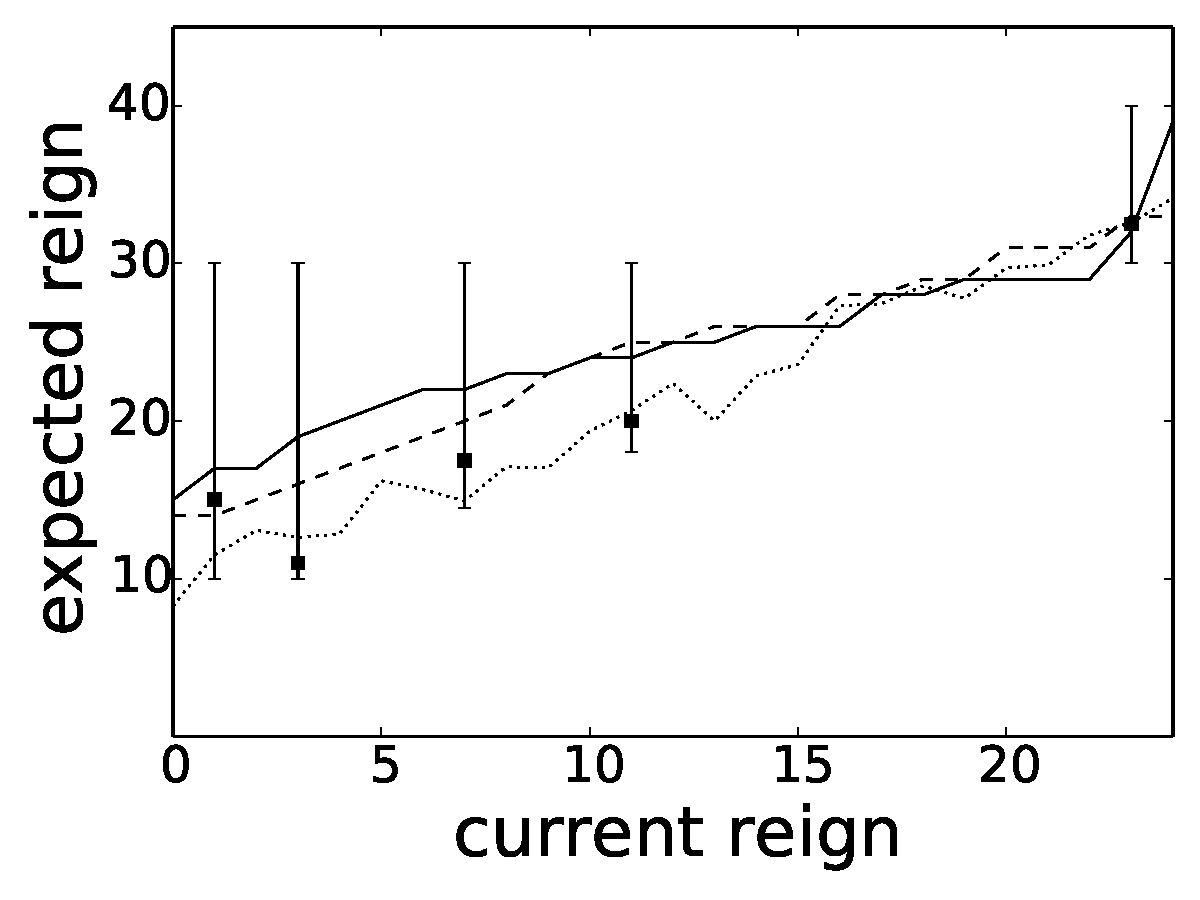
\includegraphics[width=1.0\textwidth]{predictions_figures/pharaohs_reigns_pred.pdf}
	\end{subfigure}
	\begin{subfigure}{.33\textwidth}
		\caption{Movie runtimes}
		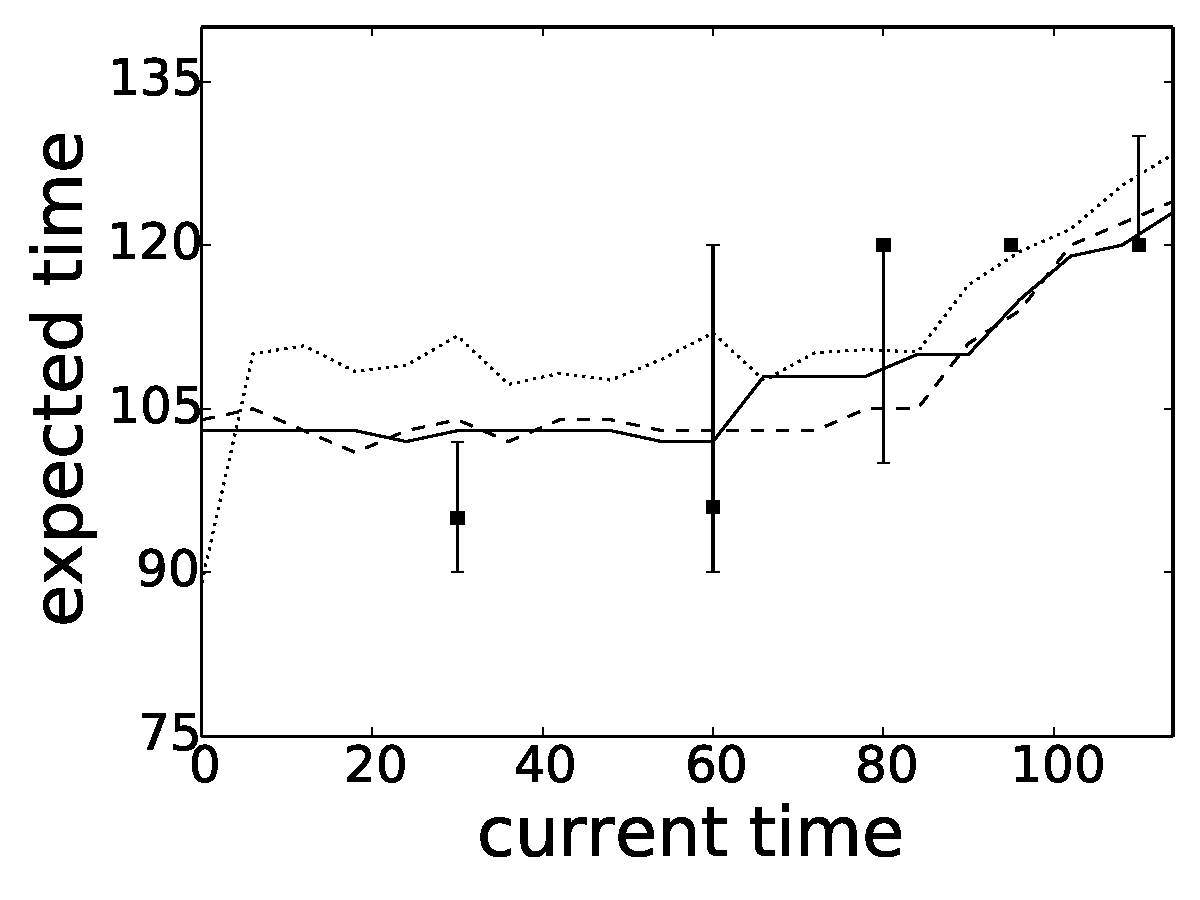
\includegraphics[width=1.0\textwidth]{predictions_figures/movie_runtimes_pred.pdf}
	\end{subfigure}
	\begin{subfigure}{.33\textwidth}
		\caption{Representatives}
		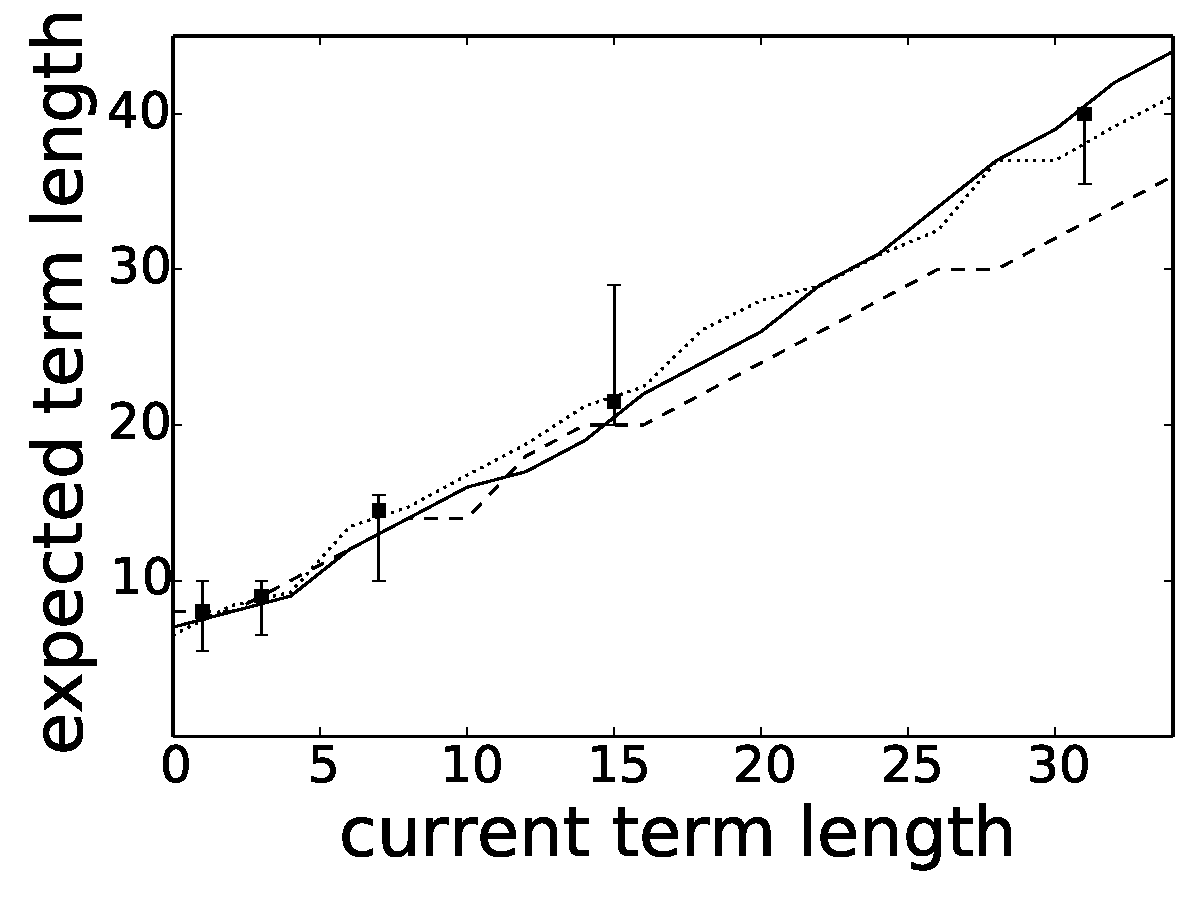
\includegraphics[width=1.0\textwidth]{predictions_figures/representatives_terms_pred.pdf}
	\end{subfigure}
	}\\
		
	\caption{Replication of the optimal predictions study from GT2. Square markers plot the median empirical response to every question, with error bars plotting bootstrapped $95\%$ confidence intervals. The dashed lines show the posterior median value of $t$ predicted using the optimal predictions model, solid lines show the median posterior predictive responses from the Noisy \mink model, and the dotted lines represent the median posterior predictive responses by the data-driven Bayesian model. All models show good qualitative predictions, with the Noisy \mink fitting the data better than the two Bayesian models.}
	\label{fig:emp_vs_mink_agg_predictive}
\end{figure}
        





\begin{table}
\centering
\begin{threeparttable}
    \caption{Quantitative measures of model fit to the replication of GT2, using normalized root mean squared error (NRMSE). The Noisy \mink model consistently has the lowest NRMSE scores: assessed solely in terms of the ability to mimic the empirical data it outperforms both of the Bayesian models.}
    \begin{tabular}{llll}
      \toprule
		& \multicolumn{3}{c}{NRMSE}\\
		\midrule
        Question & optimal Bayes & Noisy \mink & descriptive Bayes\\
        \midrule
        Movie grosses & 0.20 & \textbf{0.15} & 0.46\\
		Poem lengths & 0.55 & \textbf{0.10} & 0.19\\
		Lifespans & 0.20 & \textbf{0.10} & 0.66\\
		Pharaohs' reigns & 0.47 & 0.63 & \textbf{0.29}\\
		Movie runtimes & 0.78 & \textbf{0.61} & 0.92\\
		Representatives & 0.24 & 0.10 & \textbf{0.08}\\
      \midrule
    \end{tabular}
    \begin{tablenotes}
      \small
      \item \textit{Note.} The scores with the best results for each question are shown in bold.
    \end{tablenotes}
\label{tbl:nrmse_comparison}
\end{threeparttable}
\end{table}


\bigskip
\subsubsection{Generalizability to new data}

The problem with using descriptive adequacy as the sole measure of model performance is that it is unable to detect overly elaborate models \cite<e.g.,>{myung_importance_2000}. Attempts to correct for model complexity by counting the number of free parameters such as AIC or BIC improve on this a little, but not much. The optimal predictions model produces parameter-free predictions, the Noisy \mink model uses four parameters, and the descriptive Bayesian model uses five. If model evaluations could be safely made by looking only at the number of parameters and the goodness of the data fit, we ought to be able to safely rule out the descriptive Bayesian model: it has more parameters than Noisy \mink and yet produces a worse fit. As it turns out, this intuition is wrong. 

To understand why this intuition is incorrect, we consider an alternate method of quantitative comparison known as cross-validation---a standard technique from the model selection literature \cite{browne_cross-validation_2000}---although other options are available such as Bayes factors \cite{wasserman2000bayesian} or approaches specifically geared towards evaluating optimal models using information theory \cite{shen2016}. The central goal in model selection is generally assumed to be to pick the model that will make the best predictions about out-of-sample data, and cross-validation aims to approximate this by estimating parameters on one subset of the empirical data and evaluating performance by measuring how well the model fits capture the held-out data. 

To see how all three models generalize to new data, we trained using only a subset of our empirical data, and then tested the models by assessing how well the inferred priors allowed the models to generalize to the withheld data. Specifically, we used $k$-fold cross validation with $k=25$, which involves partitioning the original data set into 25 similarly-sized sub-samples\footnote{For each repetition of the process, between 3 and 5 data points were withheld, with a maximum of one response from a single individual per repetition. The repetitions were balanced so that each data point was withheld exactly once in the entire cross-validation procedure.} and treating each sample once as the unobserved data and the other 24 as the training data. This provides a robust estimate of how each model generalizes to unobserved data.  

The results are shown in Table \ref{tbl:cross_validation}. The descriptive Bayesian model has the best overall performance, outperforming the optimal Bayesian model and Noisy \mink in every case. Moreover, although the qualitative comparison in the previous section suggested that Noisy \mink provided a reasonable fit to the data, it performed very poorly in cross validation, far worse than either of the Bayesian models. Despite the apparent simplicity of the Noisy \mink heuristic, it actually corresponds to an overly flexible statistical model for the data. The Noisy \mink model overfits the training data and generalizes poorly to new observations. In contrast, the apparent complexity of the optimal Bayesian model as a psychological theory hides the fact that when viewed as a statistical model for empirical data it is insufficiently flexible, and ends up underfitting the data. The descriptive Bayesian model outperforms them both.


\begin{table}
\centering
\begin{threeparttable}
    \caption{Cross validation model comparisons. In all domains, the data-driven Bayesian model generalizes to new data better than either of the other two models.}
    \begin{tabular}{llll}
      \toprule
		& \multicolumn{3}{c}{Cross validation score}\\
		\midrule
		 & optimal Bayes & descriptive Bayes  & Noisy \mink \\
      \midrule
        Movie grosses & -713 & \textbf{-150} & -100886\\
		Poem lengths & -118 & \textbf{-116} & -3762\\
		Lifespans & -526 & \textbf{-187} & -2327\\
		Pharaohs' reigns & -132 & \textbf{-103} & -2380\\
		Movie runtimes & -258 & \textbf{-153} & -6786\\
		Representatives & -174 & \textbf{-97} & -511\\
		Future lifespans & - & \textbf{-188} & - \\
		Waiting times & - & -91 & - \\
		%\midrule
		\textbf{Average} & -320 & \textbf{-135} & -19442\\
      \midrule
    \end{tabular}
    \begin{tablenotes}
      \small
      \item \textit{Note.} Higher scores (lower absolute values) indicate better generalization. The best score in each row is shown in bold. The bottom row shows the average score for each model across question types. In order to be comparable to the other models, the average score for the data driven Bayesian model is based on the first six rows only.
    \end{tablenotes}
\label{tbl:cross_validation}
\end{threeparttable}
\end{table}

\bigskip
\subsubsection*{Comparing subjective priors to optimal ones}

So far we have seen that, although the descriptive Bayesian framework led us to specify a flexible, statistically complex model, this complexity was justified insofar as this model generalizes to new data better than either the original Bayesian model or the Noisy \mink heuristic. This suggests that there are sound statistical justifications for preferring the descriptive Bayesian model. 

However, from a theoretical and psychological perspective, it is not sufficient merely to show that a model is statistically superior to its competitors: A good model should also explain why people behave the way they do. In this respect it is the {\it contrast} between the optimal priors in the GT2 model and the inferred priors extracted by our model that is especially useful. This comparison is shown in Figure \ref{fig:predictions-priors-subjective-vs-empirical}, and is instructive both in terms of the similarities and the differences in reveals. Inspection of this figure suggests that although people's subjective priors are similar to the true environmental distributions, there are systematic deviations in most cases: People's prior expectations about movie run times and representative term lengths both seem to be too long, and their beliefs about lifespan distributions seem to underestimate infant and child mortality rates.\footnote{Note that the latter may be partly due to the limitations of the experimental design and the model, given that the model does not make it easy to estimate negatively skewed distributions and the experiment does not ask questions that tease apart people's beliefs about infant mortality.} The distribution of future lifespans does not have a veridical value, but the descriptive model infers something that seems sensible: It has a similar form to the subjective prior for actual life spans, but is shifted to the right with an average life span of 105. That said, in spite of the minor differences the overall degree of agreement between the two Bayesian models is remarkable, especially given that the built in assumptions about participant priors in the descriptive model were fairly weak.


\begin{figure}[t]
	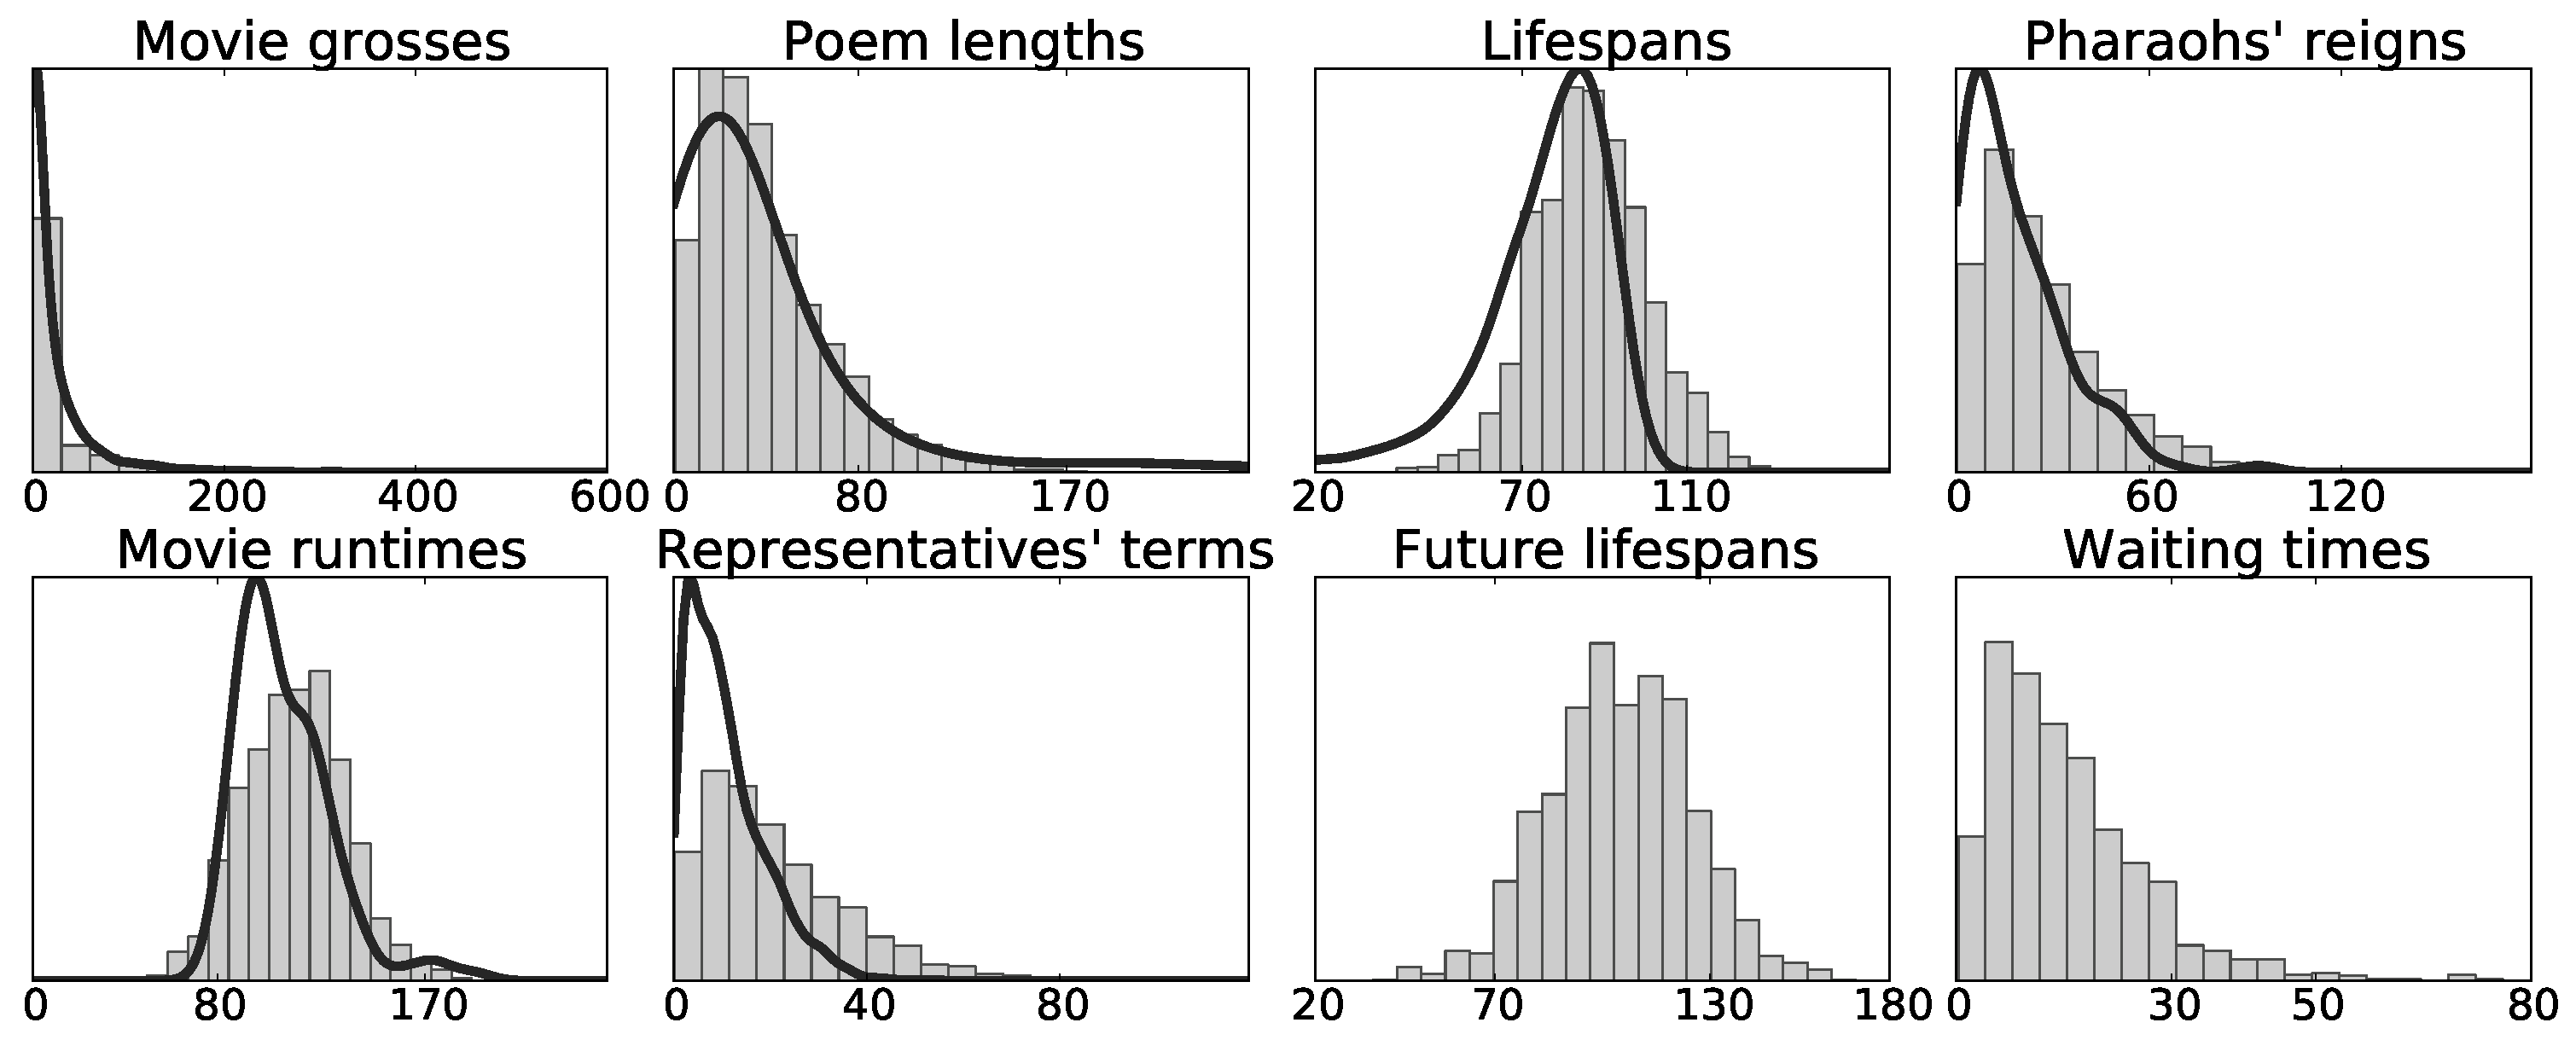
\includegraphics[width=1.0\textwidth]{predictions_figures/priors-subjective-vs-empirical.pdf}
	\caption{Estimates of people's subjective prior beliefs (histograms) compared with the environmental distributions collected by GT2 (lines). In most cases the estimates are similar to the true distributions, although people often underestimate the frequency of events at lower numbers. There was no environmental data available for future lifespans and waiting times.}
	\label{fig:predictions-priors-subjective-vs-empirical}
\end{figure}



\subsection*{Discussion}

Whereas the take-home point from the first case study was that descriptive Bayesian models can be psychologically revealing even when optimal Bayesian models are wrong, the second case study tells a very different story, one in which the exploratory and data-driven analysis based on descriptive Bayesian models complements the original optimal Bayesian model.  Although the optimal predictions model from GT2 is not the best performing model either in terms of the data fit (Noisy \mink is best) or generalizability (descriptive Bayes is best), we found it almost impossible avoid the conclusion that the original rational analysis was remarkably successful.  It is true that the estimated priors plotted in Figure~\ref{fig:predictions-priors-subjective-vs-empirical} do show systematic differences from the optimal ones, which explains why the optimal predictions model does not win in the model selection exercise. These deviations, which we would not have known about without the descriptive Bayesian model, are cognitively interesting; but even so, the similarities between the estimated priors and the veridical ones are much more striking than the differences. 

In this instance, the descriptive Bayesian approach reinforces the conclusions from the original rational analysis. Indeed, because of the descriptive Bayesian approach, we feel far {\it more} confident in drawing conclusions about (near-)optimality than we did based on the optimal model only: The descriptive model was afforded the freedom to choose whatever prior distribution (from a very broad family) best accommodated the empirical data, but the end result was a collection priors that are only very slightly different to the veridical ones used by GT2. In our view this provides much stronger evidence for optimality than the original analysis, which showed a qualitative agreement between the optimal model and empiricial data but did not include any formal model comparisons.

When contrasting the descriptive and optimal Bayesian approaches, it is worth noting that {\it any} choices made by researchers are going to incorporate biases of some sort. After all, we have to make {\it some} assumptions about the family of priors people might have, or the type of likelihood functions, and so forth. For example, the assumptions that we built in to the descriptive model were shaped by previous research and our own goals as researchers. We are not arguing that the descriptive approach cannot fall prey to these problems; they are an inevitable part of doing science within any modeling framework.  However, the descriptive Bayesian approach (a) allows us to build in fewer assumptions---e.g. a family of distributions allows for many more possibilities than a single one---and (b) more importantly, does not require that those assumptions be justified on the basis of optimality. GT2 were forced by the straightjacket of optimal Bayesian modeling to have to claim that the distributions they chose were justified on the basis that they were well-matched to the real world. We were forced to make no such claim; we simply chose a family of distributions based on what was sensible and then observed which of those best fit the pattern of human performance.

Of course, some cautionary notes should be attached to these results. For instance, to avoid covering the same ground as the first case study we have not developed a Bayesian model that accounts for individual differences. Similarly, our discussion of the Noisy \mink model in this section has been more cursory than the model deserves purely because our focus is on different kinds of Bayesian models. As an example, our data analysis automatically produces estimates of the multiplier parameter $g$ as well as specific exemplars that the Noisy \mink model uses to generate responses. Other variations on Noisy \mink might perform better, and we do not think strong conclusions about the relative merits of Bayesian and heuristic models should be drawn from these analyses. Even so, the model comparisons here highlight the manner in which it is possible to make sensible comparisons between optimal Bayesian models, non-optimal heuristic models, and descriptive Bayesian models, so long as good statistical procedures are used to guide the comparison.




